\documentclass[a4paper, 10pt]{article}
\usepackage[utf8]{inputenc}
\usepackage{verbatim}
\usepackage{float}
\usepackage{listings}
\usepackage{graphicx}
\usepackage{a4wide}
\usepackage{color}
\usepackage{amsmath}
\usepackage{amssymb}
\usepackage[dvips]{epsfig}
\usepackage[toc,page]{appendix}
\usepackage[T1]{fontenc}
\usepackage{cite} % [2,3,4] --> [2--4]
\usepackage{shadow}
\usepackage{hyperref}
\usepackage{titling}
\usepackage{marvosym }
\usepackage{physics}
\usepackage{subcaption}
\usepackage{booktabs}
\usepackage{microtype}
\usepackage{ifthen}
\usepackage{tikz}
\usetikzlibrary{shapes,arrows}
\usepackage[noabbrev]{cleveref}
\usepackage{wasysym}
\usepackage{changepage}

\newcommand{\gray}[1]{\textcolor{gray}{#1}}
\newcommand{\spin}[1]{\ifthenelse{#1 = 1}{\uparrow}{\downarrow}}
\newcommand{\tilstand}[4]{
    \(\displaystyle
        \begin{matrix}
                & \gray{\spin{#3}} & \gray{\spin{#4}}\\
            \gray{\spin{#2}} & \spin{#1}  & \spin{#2} & \gray{\spin{#1}}\\
            \gray{\spin{#4}} & \spin{#3} & \spin{#4} &  \gray{\spin{#3}}\\
                & \gray{\spin{#1}} & \gray{\spin{#2}}
        \end{matrix}
    \)
}

\renewcommand{\topfraction}{.85}
\renewcommand{\bottomfraction}{.7}
\renewcommand{\textfraction}{.15}
\renewcommand{\floatpagefraction}{.66}
\renewcommand{\dbltopfraction}{.66}
\renewcommand{\dblfloatpagefraction}{.66}
\setcounter{topnumber}{9}
\setcounter{bottomnumber}{9}
\setcounter{totalnumber}{20}
\setcounter{dbltopnumber}{9}


\setlength{\droptitle}{-10em}   % This is your set screw

\setcounter{tocdepth}{2}

\lstset{language=c++}
\lstset{alsolanguage=[90]Fortran}
\lstset{basicstyle=\small}
\lstset{backgroundcolor=\color{white}}
\lstset{frame=single}
\lstset{stringstyle=\ttfamily}
\lstset{keywordstyle=\color{red}\bfseries}
\lstset{commentstyle=\itshape\color{blue}}
\lstset{showspaces=false}
\lstset{showstringspaces=false}
\lstset{showtabs=false}
\lstset{breaklines}
\title{
Study of phase transisition in finite size magnetic systems using 2D Ising model}
\author{Aram Salihi$^1$\\
  \small $^1$Department of Physics, University of Oslo, N-0316 Oslo, Norway}
\begin{document}
\maketitle
\begin{abstract}
In this numerical study we are going to use the two dimensional Ising model to investigate
how different thermodynamical quantities behave. The main interest and the goal of this
study is to look at the behaviour of large system when reaching the Curie temperature, and compare the numerical
Curie temperature with the analytical solution found by Onsager \cite{morten}. In this article we have
analytically solved the two dimensional Ising for $2\times2$ lattice, and numerically solved for lattices with spins $L = \{40,60,80,100,120\}$.
The study where successful, and we obtained a estimation of the Curie temperature to be $T_{C} = 2.24 \pm 0.029$ with a
relative error $1.278\%$ which is quite acceptable.
\end{abstract}
\tableofcontents

\section{Introduction} The Ising model is a simple but very elegant theory which describes the
behaviour of ferro- and anti-ferromagnets in materials, and is widely used in statistical physics to get a better understanding of different thermodynamical quantitites.
The model consist of a lattice where each points represent
a dipole with configruation $+1,-1$. The energy of the lattice is described by
the sum of interal magnetic moment interaction between neighbouring dipoles.  This Ising model has analytical solutions
for one and two dimensions, but analytical solutions for higher dimensions are yet not been discovered due to complexity
which occours in the system. The solution for one dimension were derived by the German physicist Ernst Ising, and also concluded
that phase transitions does not exist in the Ising model, he also further concluded that phase transition does not exist for
higher dimension. This was later proven to be wrong by the famous Norwegian theoretical physcist and chemist Lars Onsager.
He showed that an analytical solution does exist and the Ising model unders goes second order phase transition when
approaching the Curie temperature \cite{noe} for infintely large lattice. After this critical point, the lattice looses the ability of self magnetize and becomes
a paramagnet.
\vspace{3mm}
\\
For finite lattice sizes for large system the problem becomes more complex and impossible to find a solution.
Since the lattice system described in the Ising model is microcanonical it follows Boltszmann statistics,
the problem arises in the partition function. The partition function need all possible configruations of the lattice, which goes as $2^{N}$,
in order to calculate the probability function. Since we know that probability distribution do exist, we can use
the Metropolis algorithm to solve this problem for finite lattice sizes.  The beauty of this algorithm is that its not
dependent on the parition function, but only the acceptance ratio from different states calculated by the boltzmann factor.
In this project we are going to use the Metropolis algorithm to investigate different thermodynamical quantities and the phase transition
in the two dimensional Ising model and try to estimate the Curie temperature. We are going to use this estimation to compare with analytical
solution found by Onsager \cite{morten} for inifinetly large lattice.

\section{Mathemetical and physical theory \label{theory section}}
\subsection{Ising model \label{ising model}} As mentioned in the introduction we will be looking at the so called 2-Dimensional
"Ising model". The Idea is pretty simple and straight forward. Imagine having a microcanonical (fixed temperature
$T$) system consisting of a
square lattice with dimension $L\times L$. In this lattice, each points corresponds to a
particle with a magnetic dipole (which we will call for spin) . We will define the spin confiquration of a invidual
particle as
\begin{align}
  s = \{-1, + 1\}
\end{align}
The particle will either point upwards or downwards. Now each particle internal magnetic field will
have the freedom to interact with its surrounding particles. When changing a configuration, i.e
changing a arbitrary spin, the hamiltonian of the system will change
according to
\begin{align}
  H = -\mathcal{J}\sum_{\langle kl \rangle}^{N} s_{k}s_{l} + \mathcal{B}\sum_{k}^{N}s_{k}
\end{align}
Where $\mathcal{J}$ is the coupling constant which expresses the strength of the interaction
between neighbouring spins, and $\mathcal{B}$ is a external magnetic field interacting with
the current magnetic field of dipole $k$. A derivation of the hamiltonian can be found at
\cite{Michael}. We will look at a simplified case, where we assume no
external fields acting on our system, thus $\mathcal{B} = 0$
\begin{align}
  H = -\mathcal{J}\sum_{\langle kl \rangle}^{N} s_{k}s_{l}
  \label{ising energy}
\end{align}
Notice we have used the symbol $\langle kl \rangle$ to indicate that we only sum
over neighbouring spins. The magnetic moment of a certain configuration is then defined as
\begin{align}
    M = \sum_{k}^{N} s_{k}
    \label{ising magnetic}
\end{align}
Since this system is a microcanonical system it can be described perfectly with
Boltzmann statistics. For further explaination please consider \cite{valery}
\subsection{Boltzmann statistics} Suppose we have system $\mathcal{S}$ with a fixed temperature
$T$ and no interaction with its surrounding envirorment, meaning no
exchange of heat/energy. The system will keep its shape, number of particle and the total energy is conserved.
Thus, in other words we have thermal equilibrium at all time. The probability of a state or configruation $i$
for a given energy configruation $E_{i}$ (in our case $E_{i}$ is from equation
\eqref{ising energy} ), the probability distribution function is defined by
boltzmann statistics
\begin{align}
  P(E_{i}) = \frac{1}{Z}e^{-\beta E_{i}}
  \label{prob dens}
\end{align}
where $\beta = 1/(k_{b}T)$ and $Z$ is the partion function. The Partition function is easily derived, the total sum of all possible states are $1$
\begin{align}
  \sum_{i \le N} P(E_{i}) =  \sum_{i\le N} \frac{1}{Z}e^{-\beta E_{i}} = 1
\end{align}
Solving this with respect to $Z$, we will achieve
\begin{align}
  Z = \sum_{i\le N} e^{-\beta E_{i}}
\end{align}
The partion function is a another word for normalization constant. Notice that the
sum is over all microstates $i$, consisting of $N$ states.
\subsection{Expectation value} For a given energy confiquration there exist a probability distribution function $P(E_{j})$. Now if we let a general variable
$\Psi^{n}$ represent a physical quantity from this system described by $P(E_{j})$ there is
a expectation value. Using the probability distribution function and discrete points, the expression
for expectation value of $\Psi^{n}$ is then:
\begin{align}
  \langle \Psi^{n} \rangle = \sum_{j \le N} \Psi^{n}P(E_{j}) = \frac{1}{Z}\sum_{j \le N} \Psi^{n}
  e^{-\beta E_{j}}
  \label{expect val}
\end{align}
This expression will become very handy as we are going to derive analytical expression for
important thermodynamical quantities.

\subsection{Thermodynamical quantitites} By using the ising model we wish to
calculate different thermodynamical quantitites, to see how the system behave for different temperatures,
and how the change is from one phase to another.
The quantitites we wish to calculate is heat capacity and magnetic Suscepbility.
\subsubsection{Heat Capacity} The definition of heat capacity is
\begin{align}
  C_{v} = \pdv{\langle E \rangle}{T} = \pdv{T}\left(\pdv{\beta}\ln{Z}\right)
\end{align}
For the sake of simplicity in our numerical calculation we will not use the above definition. Since we are
using discretized points, we will therefore use the following expression (which is equivalent)
\begin{align}
  C_{v} = \frac{\mathrm{Var}(E)}{kT^{2}} =\frac{\langle E ^{2} \rangle - \langle E \rangle^{2}}{kT^{2}}
\label{heat capacity}
\end{align}
Where $\langle E ^{2} \rangle$ is the expectation value of squared energy and $\langle E \rangle$ is the expectation value of energy.
The fully derivation of the heat capacity is given
in the appendix \eqref{heat capacity}.
\subsubsection{Magnetic susceptbility} The definition of magnetic susceptbility is
\begin{align}
  M = \pdv{\langle M \rangle}{B} = \frac{1}{\beta}\pdv{B}\left(\pdv{\beta}\ln{Z}\right)
\end{align}
Where $B$ is the magnetic field strength of spin $i$. It is crucical to not
mix $\beta$ and $B$, $\beta$ represent unit of energy per kelvin and $B$ is magnetic field stength in teslas $T$.
Again for the sake of simplicity we will not choose to use the above expression, we will therefore
derive another expression which is equivalent to the expression above. Consider the following
\begin{align}
  \chi = \frac{\mathrm{Var}(M)}{kT} =
  \frac{\langle M ^{2} \rangle - \langle M \rangle^{2}}{kT}
  \label{magsus}
\end{align}
The fully derivation of this expression is given in the appendix \eqref{magnetic susceptibility}.
\subsection{Analytical solution for  $2\times 2$ lattice \label{2x2 analytical}} Assume a system with number of spins equal to $L =2$
in a  $2\times 2$ square lattice. We have total of four spins,
where each spin have two spin orientation, $\{+1,-1\}$. Meaning we have $2^{4} = 16$
lattice configruations. Using periodic boundary conditions we will obtain these lattice configruations states
\begin{center}
  $1.$\tilstand{0}{0}{0}{0} \quad
  $2.$  \tilstand{0}{0}{0}{1} \quad
  $3.$  \tilstand{0}{0}{1}{0} \quad
  $4.$  \tilstand{0}{0}{1}{1} \quad
  \vspace{3mm}
  \\
  $5.$  \tilstand{0}{1}{0}{0}\quad
  $6.$  \tilstand{0}{1}{0}{1} \quad
  $7.$  \tilstand{0}{1}{1}{0} \quad
  $8.$  \tilstand{0}{1}{1}{1} \quad
  \vspace{3mm}
  \\
  $9.$  \tilstand{1}{0}{0}{0} \quad
  $10.$  \tilstand{1}{0}{0}{1} \quad
  $11.$  \tilstand{1}{0}{1}{0} \quad
  $12.$  \tilstand{1}{0}{1}{1} \quad
  \vspace{3mm}
  \\
  $13.$  \tilstand{1}{1}{0}{0} \quad
  $14.$  \tilstand{1}{1}{0}{1} \quad
  $15.$  \tilstand{1}{1}{1}{0} \quad
  $16.$  \tilstand{1}{1}{1}{1}
\end{center}
Using the energy given in \eqref{ising energy}  in section \eqref{ising model} the lattice system will have these five possible energy states
\begin{center}
  \begin{table}[H]
    \centering
    \begin{tabular}{cccc}\toprule
        Number of \(\uparrow\) & Multiplicity & Energy & Magnetic moment\\ \midrule
        \(4\) & \(1\) & \(-8J\) & \(4\) \\ \midrule
        \(3\) & \(4\) & \(0\) & \(2\) \\ \midrule
        \(2\) & \(2\) & \(8J\) & \(0\) \\ \midrule
        \(2\) & \(4\) & \(0\) & \(0\) \\ \midrule
        \(1\) & \(4\) & \(0\) & \(-2\) \\ \midrule
        \(0\) & \(1\) & \(-8J\) & \(-4\) \\ \bottomrule
    \end{tabular}
\end{table}
\end{center}
The partition function for these configruations becomes
\begin{align}
  Z = \sum_{i = 1}^{16}e^{-\beta E_{i}} = 2e^{8\beta J} + 2e^{-8\beta J} + 12 = 4\cosh{\left(8\beta J\right)} + 12
\end{align}
The probability distribution function for this system becomes for a lattice in state $j$ with energy $E_{j}$
\begin{align}
  P(E_{j}) = \frac{e^{-\beta E_{j}}}{4\cosh{\left(8\beta J\right)} + 12}
\end{align}
Now that we have an analytical expression for the partition for all possible configurations
of the lattice, we can now derive analytical expression for $C_{v}$, $\langle |M|\rangle$ and $\chi$.
\subsubsection{Heat capacity}
In order to calculate the heat capacity we need the mean expaction value, $\langle E \rangle$,
and the expectation value of sqaured energy, $\langle E^2 \rangle$. Using the general expression for expectation value
\eqref{expect val}, thus
\begin{align}
  \langle E \rangle = \frac{1}{Z}\sum_{i}^{16}E_{i}P(E_{i}) = -\frac{8J\sinh{(8\beta J)}}{\cosh{\left(8\beta J\right)} + 3}
\end{align}
and the squared energy
\begin{align}
  \langle E^{2} \rangle = \frac{1}{Z}\sum_{i}^{16}E^{2}_{i}P(E_{i}) = \frac{64J^{2}\cosh{(8\beta J)}}{\cosh{\left(8\beta J\right)} + 3}
\end{align}
Using the analytical expression \eqref{heat capacity} presented in previous section, the solution of the heat capacity
becomes
\begin{align}
  C_{V} = \frac{\mathrm{Var}(E)}{kT^{2}} =\frac{1}{kT^{2}} \left(
  \frac{256J^{2}\cosh{(8\beta J)}}{4\cosh{\left(8\beta J\right)} + 12} -
  \left(\frac{8J\sinh{(8\beta J)}}{4\cosh{\left(8\beta J\right)} + 12}\right)^{2}
  \right)
\end{align}
\subsubsection{Magnetic susceptibility} Again using the same approach as previous, the partition function
still remains the same. The expectation value of the magnetic moment is given as
\begin{align}
  \langle M \rangle = \frac{1}{Z}\sum_{i}^{16}M_{i}P(E_{i}) = 0
\end{align}
and the squared magnetic moment
\begin{align}
  \langle M^{2} \rangle = \frac{1}{Z}\sum_{i}^{16}M^{2}_{i}P(E_{i}) = \frac{8e^{8\beta J} + 8}{3\cosh{\left(8\beta J\right)} + 3}
\end{align}
Using this and the analytical expression from \eqref{magsus}, the magnetic susceptibility becomes
\begin{align}
  \chi  = \frac{\mathrm{Var}(M)}{kT} = \frac{1}{KT}\frac{8e^{8\beta J} + 8}{3\cosh{\left(8\beta J\right)} + 3}
\end{align}
\subsubsection{Expectation value of absolute magnetic moment} Recall from previous that the expectation value
for $M$ were zero. We are now interest if $|M|$ has a explicit expression. As before using the definition
of the expectation value, the expectation value of absolute magnetic moment is given as
\begin{align}
  \langle |M| \rangle = \frac{1}{Z}\sum_{i}^{16}|M|_{i}P(E_{i}) = \frac{2e^{8\beta J} + 4}{3\cosh{\left(8\beta J\right)} + 3}
\end{align}

\subsection{Phase transisition \label{phase transition}} As explained in \cite{stat} there is no phase transitions in the one dimensional
ising model since due to never achieving a ordered confiquration of the system.
This means that the lattice remains
as a ferromagnetic system for $\beta$. As proven later by the famous Norwegian
theoretical physcisit and chemist, Lars Onsager, proved that there exist
phase transitions (for second order phase transition please check \cite{landau}) in two dimensional Ising model when reaching the curie tempeature \cite{morten}.
 Meaning that for a random confiqurated square lattice
(with no external magnetic field exterted on it)
for low temperatures the system will be in a ferromagnetic state until
it has reached the curie temperature where it undergoes a second order phase transition
and become paramagnet where it looses its ability to self magnetize.
Near this critical or so called curie temperature, $T_{C}$, we can use simple power law approximation to show
how different thermodynamical quantities behave. Consider the following mean expressions
\subsubsection{mean magnetization}
\begin{align}
  \langle M(T) \rangle \sim |T_{C} - T|^{\beta}
\end{align}
Where $\beta = 1/8$. A similar relation can applies also for the heat capacity and magnetic susceptbility
\subsubsection{Heat capacity}
\begin{align}
  C_{V} \sim  |T - T_{C}|^{\alpha}
\end{align}
Where $\alpha = 0$
\subsubsection{Heat capacity}
\begin{align}
  \chi \sim  |T - T_{C}|^{\gamma}
\end{align}
$\gamma = 7/4$. The exponent $\alpha, \beta,\gamma$ are the so-called critical exponents.
The Curie temperature is heavily depended on the lattice size i.e number of spins/particles, when increasing the
the number of spins $L$ and the curie temperature $T_{C}$ converges to a certain value when $L \to \infty$.
Ideally this is imposible to achieve numerically since our computational capacity is up to $L = 140$, but have chosen only
do simulations from $L = 2$ to $L =100$ to save time. The beauty is that we can estimate the Curie temperature
through so-called finite scale sizing relations it is possible to relate the behaviour of
finite and infintely large lattice. The Curie temperature scales then as
\begin{align}
  T_{C}(L) - T_{C}(L\to \infty) = aL^{-1/\nu}
  \label{curie temp relation}
\end{align}
Where $\nu$ can be calculated from $\xi \sim |T_{c}-T|^{-\nu}$ and $a$ is some constant.
In order to find a estimate for $T_{C}(L)$ we must find out what the constant $a$ is, to do so we can
look at the difference for two lattices $L_{1}$ and $L_{2}$. Consider
\begin{align}
  aL_{1}^{-1/\nu}-aL_{2}^{-1/\nu} = \left(T_{C}(L_{1}) - T_{C}(L_{1}\to \infty)\right) - \left(T_{C}(L_{2}) - T_{C}(L_{2}\to \infty)\right)
\end{align}
Notice when $L_{1}, L_{2} \to \infty$ there basicly identical, thus $T_{C}(L_{1}\to \infty) = T_{C}(L_{2}\to \infty)$.
This will cancel each other out. Solving with respect to $a$, we will obtain the following expression
\begin{align}
  a = \frac{T_{C}(L_{1}) - T_{C}(L_{2})}{L_{1}^{-1/\nu}-L_{2}^{-1/\nu}}
  \label{a}
\end{align}
Using this expression for $a$ in \eqref{curie temp relation}, and solve it for $L(L\to \infty)$
\begin{align}
  T_{C}(L\to \infty) =T_{C}(L) -  \frac{T_{C}(L_{1}) - T_{C}(L_{2})}{L_{1}^{-1/\nu}-L_{2}^{-1/\nu}}L^{-1/\nu}
\end{align}
The Curie temperature can be observed when we observe a breaking point.
The second order phase transition are characterized by a divergent magnetic susceptibility and heat capacity.
A analytical solution has been achieved for $\nu$ by Lars Onsager, for further explaination please read \cite.
The analytical solution Lars Onsager found is on the form:
\begin{align}
  T_{C}(L \to \infty) = \frac{2}{\ln{(1 + \sqrt{2})}}\approx 2.269
\end{align}
\subsection{Periodic boundary condition \label{periodic theory}} To avoid problems at the boundary we will assume that we have a crystal
which is infinitely large, but in reality there is no such things. So in order to bring out this affect
we let particles on the boundary interfere with particle on the oposite end, we will then achieve a
continous force/field exchange and avoid discontinuities. In this project we will be only looking at a slice of this crystal
with dimension $L\times L$ as mentioned previously sections. A expression for this is derived and illustraded
in section \eqref{periodic method}
\subsection{Metropolis algorithm \label{metropolis theory}}
Suppose having a system in a random spin confiquration $i$ and we wish to find out it evovles with
time and how it reaches steady state. The problem is we do not how we can oriante the different spins
to reach equilibrium, thus the system is not deterministisc. The positivie thing is that the system
can be described with a probability density function $P(E_{i})$ for configruation $i$. Using the probabilistic nature
of this system, we can use Monte Carlo simulation to see how the system evovles with time. Once the probability
density function is known we can take random samples from it and proceed the simulation.
\vspace{3mm}
\\
Many simulation are then performed until a desired result is found. The solution of the problem will then be the result found normalized according to number
Monte Carlo used.  Now Monte Carlo simulation is not a specific algorithm, but rather a set of algorithm which uses
this idea. For further detailed explaination please consider \cite{morten}. The downfall is that we cannot choose all Monte carlo methods for this project, because computing the partion function $Z$ for large system is quite impossible.
It is not possible to calculate all spin oriations for large system.
We must then develop a algorithm which bypasses this problem. One of the Monte Carlo methods bypasses this problem.
The beauty of the
Metropolis algorithm is that we only look at the probability ratio of two different energy states, the so called acceptance ratio, dentoed as $A_{i\to j}$. Meaning we are looking at a lattice in some state jumping to another state,
by flipping a random spin $\mathcal{S}$. Thus
\begin{align}
  A_{i \to j} = \frac{P(E_{j})}{P(E_{i})} = \frac{e^{-\beta E_{j}/Z }}{e^{-\beta E_{i}/Z}}
  = e^{-\beta(E_{j} -E_{i})} = e^{-\beta\Delta E}
\end{align}
As we see the partion function cancels out, thus we bypass this problem we initially had. In
order to accept this jump and update the thermodynamical quantitites, the acceptance ratio $A_{i \to j}$ must be lower than a random number $\zeta$
\begin{align}
  \zeta \le e^{-\beta\Delta E}
  \label{accept}
\end{align}
This number is defined by a uniformal random distribution in the interval $[0,1]$. If
\begin{align}
    \zeta > e^{-\beta\Delta E}
\end{align}
Then we cannot accept the change of state, and we must continue to choose a random spin
and flip it, and then again check if the new configruation satisfies \eqref{accept}.
How this algorithm is implemented and simplified is explained in section \eqref{metro meth}.

\subsection{Thermodynamical equilibrium for the lattice system \label{law of large numb}} Since we are dealing with probalistic system,
a fundemental theorem probability theory states that \cite{stat}; Performing the same experiment for a large amount of cycles,
the deviation will after a while die out and the system and the average of the result normalized will tend to
the expectation value, and converge to it if sufficiently amount cycles is provided. Meaning if we find the number of Monte Carlo
cycles, $10^{N}$, needed to achieve equilibrium. This value can be found when simulating for small lattice system and see when the different
quantities converge. We can use this value at all time when running simulations for larger systems. This will save a tremendious amount of time, since
we are reducing the computational time and calculations by some factors at the same time achieving good precision for different thermodynamical quantities.
\section{Method} In this section, we will explain how the theory is implented and used as method
in the project. The theory behind these method are explained in the previous section.
\eqref{theory section}
\subsection{Periodic boundary \label{periodic method}} Using the knowledge from section \eqref{periodic theory} we can easily derive a
expression the boundary condition by using modular division. Choose a random spin $\mathcal{S}$ which has a position
at $(x_{i}$,$y_{i})$. We know that this spin will be affected by neighbouring spin at position $(x_{i+1}$,$y_{i+1})$
and $(x_{i-1}$,$y_{i-1})$. However, if this spinn, $\mathcal{S}$, has the position $(x_{boundary}$,$y_{boundary})$,
it will be affected by the spin on the opposite of the lattice as explained previously. Meaning either left or right most or top or bottom most particle.
Using this intuition we can derive a simple and elegent expression which finds the particle that affects spinn
$\mathcal{S}$, thus
\begin{align}
  i_{} = (i + N + \xi)\mathrm{mod} N
\end{align}
Where $i$ is the current index position of $\mathcal{S}$, $N$ is the number of spins (not total) and $\xi$ chooses direction (left,right, up or down) we want to look at.
Notice if $i = N$ then $i_{new} = 0$, which means that spin $\mathcal{S}$ with index $i = N$ is affected by another particle with index position
$i_{new} = 0$. Using this we will have no problem computing the new confiquration energy when flipping spin
$\mathcal{S}$. A diagram of this idea is shown down below.
\begin{center}
\begin{tikzpicture}
  \foreach \x in {0,1,2,3,4}
    \foreach \y in {0,1,2,3,4}
      {
        \draw (\x,\y) circle (0.2cm);
        \fill (\x,\y) circle (0.1cm);
      }
  \draw (4.2,0) node[right] {$x_{\mathcal{S}}, y_{\mathcal{S}}$};
  \draw (4.2,4.2) node[right] {$x_{4}, y_{4}$};
  \draw (-0.2, 0) node[left] {$x_{0}, y_{4}$};
\end{tikzpicture}
\end{center}
 Notice that $\mathcal{S}$ is on the bottom right boundary,
 the spins which will affect $\mathcal{S}$ have the coordinates $x_{0},y_{4}$ and
 $x_{4},y_{4}$. The computation of the energy difference from one state to another
will be explained in the next section.

\subsection{Energy in the system} From subsection \eqref{ising model} the hamiltonian for some random lattice confiquration in the ising
are described as the interaction between four nearest neighbours. Now the beauty of this theory is:
 when flipping a random spin, the energy difference from the old to new confiquration is always limited to some values
due to same amount of neighbours. This means we can precalculate the acceptance ratio
\eqref{accept}. The possible value for $\Delta E$ is
\begin{align}
  \Delta E = \{-8J, -4J, 0, 4J, 8J\}
\end{align}
and the acceptance ratio
\begin{align}
  A_{i \to j} = e^{-\beta \Delta E}
\end{align}
Note that $A_{i \to j}$ have also five values depending on the temperature the lattice experiences, but this
is precalculated before the monte carlo simulation starts. This means for every cycle in the metropolis algorithm, we can simply pick a random
spin and then check which configruation the neighbouring spin are in, thereafter assigning $\Delta E$
to $A_{i \to j}$. This precomputation of the acceptance ratio will reduce the computational time to some extent.
\subsection{Metroplis algorithm \label{metro meth}} Since we have a probability distribution function, we can therefore use Metropolis algorithm. The acceptance ratio
from state $i$ to $j$ are expressed as
\begin{align}
  A_{i \to j} = e^{-\beta\Delta E}
\end{align}
Where the energy difference $\Delta E$ from configruation $i$ to $j$. Even though we know what $\Delta E$ is limited
to some values, we must still compute it for every monte carlo and lattice sweep to find $A_{i \to j}$ when flipping a random spin.
We must now choose a random spin $\mathcal{S}$ in the lattice and check the change in energy the lattice experiences, to do so
Consider the energy the old and new confiquration experiences
\begin{align}
  \Delta E = E_{j} - E_{i} = -J\sum_{k}^{4}s_{j}s_{k} + J\sum_{k}^{4}s_{i}s_{k} = J\sum_{k}^{4}s_{k}(\underbrace{s_{i} - s_{j}}_{s_{j}}) = 2Js_{j}\sum_{k}^{4}s_{k}
\end{align}
Since $s_{i}-s_{j}$ is either $1$ or $-1$ we will just redefine it to $2s_{j}$, thus
\begin{align}
    \Delta E = E_{i \to j} = 2s_{j}J\sum_{k}^{4}s_{k}
\end{align}
This sum runs over all neighbouring spin $k$'s. Now the energy difference is calculated,
just assign it to a function where $A_{i\to j}$ is precalculated and check:
\begin{align}
  \zeta \le e^{-\beta \Delta E} = A_{i \to j}
\end{align}
The implentation of this is quite easy and can be explained as an floatchart:


\tikzstyle{decision} = [ diamond, aspect=1, draw, fill=blue!20, text width=7.0em, text badly centered, node distance=3.5cm, inner sep=0pt ]
\tikzstyle{block} = [ rectangle, draw, fill=blue!20, text width=8em, text centered, rounded corners, minimum height=6em ]
\tikzstyle{line} = [ draw, -latex' ]
\begin{center}
\begin{tikzpicture}[node distance=3.8cm, auto]
\node [block] (init) {1. Initiliaze a random configuration of
                        $L\times L$ lattice} ;
\node [block, below of=init] (block-1) {Choose a random move from                                         state $i$ to $j$};
\node [block, below of=block-1] (block-2) {Compute the energy                                                 difference $\Delta E =                                              E_{j} - E_{i}$ and                                                pick a random number                                              $\zeta \in [0,1]$};
\node [decision, right of=block-2] (decision) {is $\zeta \le                                                  e^{-\beta\Delta E}$};
\node [block, right of=decision] (block-3) {Update and calculate                                              thermodynamical                                                   quantities};
\node [decision, below of=block-3](decision-1){Last Monte Carlo                                                   step?};
\node [block, above of = decision](block-4){Restart the process};
\node [block, left of = decision-1](block-5){Restart process until last Monte Carlo step is achieved};
\node [block, below of = decision-1](block-6){Update all quantities, exit program};


\path [line](init)--(block-1);
\path [line](block-1)--(block-2);
\path [line](block-2)--(decision);
%\path [line](decision)--node{no}(init);
\path [line](decision)--node{yes}(block-3);
\path [line](block-3)--(decision-1);
\path [line](decision)--node{no}(block-4);
\path [line](block-4)--(block-1);
\path [line](decision-1)--node{no}(block-5);
\path [line](decision-1)--node{yes}(block-6);

\end{tikzpicture}
\end{center}


\subsection{Number of monte carlo cycles in order achieve steady-state}
There is two way to find out how many Monte Carlo cycles we need to achieve steady state.
\begin{itemize}
  \item Plotting the different thermodynamical quantities as function of Monte Carlo cycles and
  analyze it and check when large deviation dies out.
  \item Count how many times you get accepted spins flipps and plot it as a function
  Monte Carlo cycles. When the number of accepted spin flipps get steady and coverges to a certain value.
  When this happens, it means that for each Monte Carlo cycle after it has converged it doesnt matter
  how many cycle you use it will always flipp that amount of spins.
\end{itemize}
\section{Implentation of the Ising model and the structure in C++}
In this section we will briefly explain the structure and the technicalities behind the program.
The program which simulates the Ising model consist of four classes and a main class.
\subsection{Main.cpp}
This class takes in 11 input arguments. The arguments are listed in a chronologically order
\begin{itemize}
  \item argv[1]: type string. Name of the text file that is going to be generated when the program is executed. When the program exit,
  all thermodynamical quantities are saved into this .txt file.
  \item argv[2]: type int. Number of spins $L$.
  \item argv[3]: type int. Number of Monte Carlo Cycles.
  \item argv[4]: type double. $T_{i}$, Initial temperature the lattice experiences.
  \item argv[5]: type double.  $T_{f}$, Final temperature the lattice experiences.
  \item argv[6]: type double. The stepsize, $\Delta T$, when going trough the interval
  $T_{i} \le T \le T_{f}$.
    \item argv[7]: type string. Three possible string values. Up; initializes the lattice with all spins pointing upwards.
    Down; initializes a lattice where all spins pointing downwards. Random; All spins are randomly configruated, they either point up or down.
      \item argv[8]: type string. Two possible string values, ordered or dis\_ordered, this arguments are added to the end of file of argv[1]
      when saving for each step when running the Monte Carlo simulations.
        \item argv[9]: type bool: two possible value 0 or 1. 0 indicates false, when 0 is used the program only saves the last step when executed.
        1 indicates true, the program will save each step when executed.
          \item argv[10]: type bool:  two possible value 0 or 1. 1 indicates true, when executed the program will calculates $\chi$ with
          $\langle |M|\rangle$ instead of $\langle M \rangle$. This is due to avoid fast and alot oscillations when increasing $L$. When 0 is used, the program calculates
          $\chi$ with $\langle M \rangle$.
          \item argv[11]: type bool: two possible value 0 or 1. If 1, when the program is executed the simulation result are saved into a pointer array when the system reaches equilibrium/steady state.
          When 0, the program will save every quantities to the pointer array independently if the system has reached or not reached steady state.
\end{itemize}
\subsection{quantities.cpp}
This class consist of four methods. These methods initializes the lattice confiquration when the spin configuration argument is given in Main. This class also initializes precalculates
the acceptance ratio $A_{i \to j}$ used in the Metropolis, the initial energy and magnetic moment of the system.
\subsection{solver.cpp} This class consists of two methods.
The first method is called "calculate\_nabo\_spin" which calculates the neighbouring spins when looking at the energy difference.
The second method is called metropolis  which is the method where the metropolis algorithm is implemented.
\subsection{Execute\_solve.cpp}
This class consist of one main method which takes all the input arguments from main.cpp and gives to the MPI and then executes
the solver class for desired input from main.cpp.
\subsection{dumpfiles.cpp} As the name says, this is the class where all values are dumped into. This class consist of three methods:
save\_each\_step is a method used to save each value from solver.cpp into pointer arrays. Thereafter is this send to another
method called save\_each\_file\_step where the result is normalized and different qauntites are calculated and saved to a file with .txt exstension.
The last method is called save\_last\_step, this method as the name says saves the quantities at the end of the Monte Carlo cycle and then saved.
\subsection{Parallelization with MPI} The C++ program is entirely parallelized but not perfectly optimized,
this is done in order to reduce computational time. The C++ program uses the latest MPI version. The program is mainly
executed on macbook pro with two i5 cores.
\section{Result} In this section we will present the result produced from the Monte Carlo simulation.
We will also give necessary information about parameters in order to produced the same result with same precision.
\textbf{All results are normalized with respect to total number of spins and monte carlo cycles. Thus we are looking at per spin and total spin, we can interpret this
as looking at individual spin.}
\subsection{$2\times 2$ Lattice \label{2x2 result}} The Monte Carlo simulation used $L = 2$ with different Monte Carlo cycle in the range
$N = \{10^{2}, 10^{7}\}$ to show convergence towards the analytical solution derived in section \eqref{2x2 analytical}. Note that the result are functions
of temperature with unit $kT/J$. This were done for temperatures in the range $kT/J = \{0.9,1.9\}$ with $\Delta T = 1e-3$ stepsize.

\begin{figure}[H]
  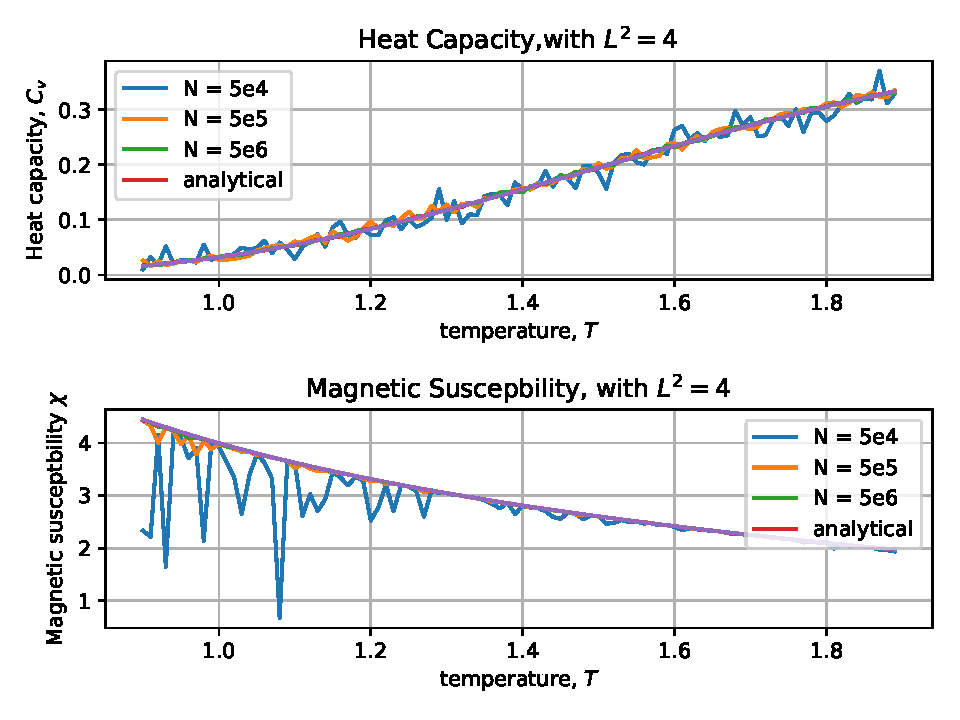
\includegraphics[width=17.0cm,height=6.3cm,keepaspectratio]{/Users/aramsalihi/Desktop/FYS4150/project4/figures/analytical_vs_numerical_2x2_magsus_and_heat_cap.pdf}
  \centering
  \caption{The diagram on the top shows the heat capacity as a function of the temperature for $L\times L = 4$, and the diagram down below
  is the magnetic susceptibility as function of temperature. Notice that these are plotted against the analytical solution.}
  \label{magsus og heatcap}
\end{figure}
We have also plotted the numerical solutions of the expectation value of the energy and absolute magnetization against their
analytical solution.
\begin{figure}[H]
  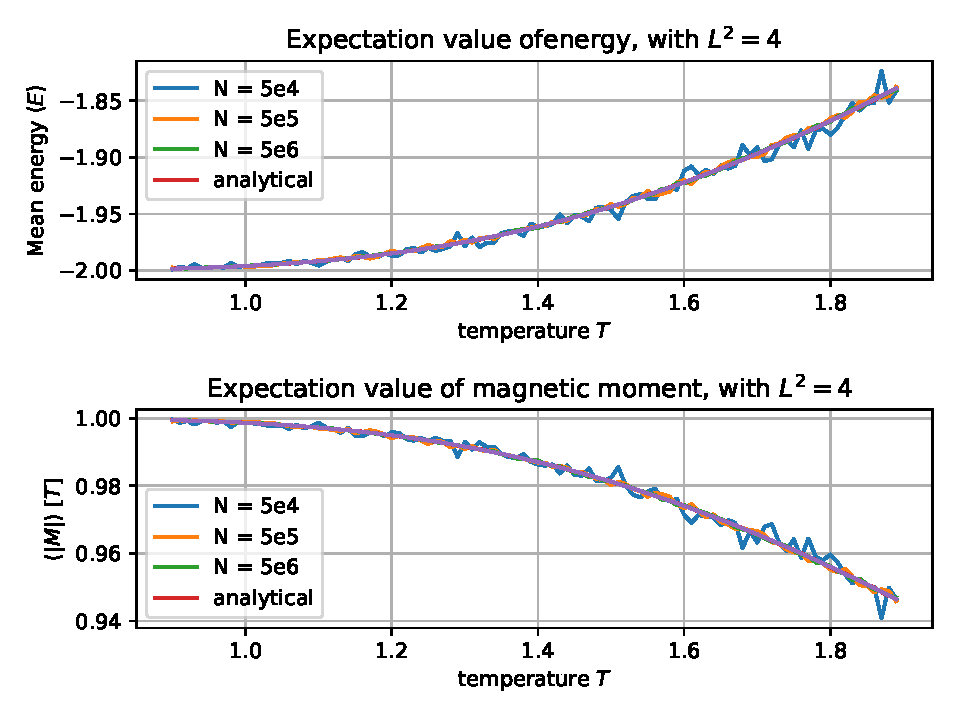
\includegraphics[width=17.0cm,height=6.3cm,keepaspectratio]{/Users/aramsalihi/Desktop/FYS4150/project4/figures/analytical_vs_numerical_2x2_mean_absmag_and_meanE.pdf}
  \centering
  \caption{The diagram on the top shows the expectation value of energy as a function of the temperature for $L\times L = 4$, and the diagram down below
  is the expectation value for absolute magnetic moment as function of temperature.}
  \label{meanE meanM}
\end{figure}
\subsection{Number of Monte Carlo needed to achieve equilibrium for $20\times 20$ lattice}
In this section we are going to present result when steady/equilibrium in our Monte Carlo simulations are achieved, this is done for  different number of Monte Carlo iteration, but also
different spin configruations. We have a chaotic disordered lattice state and one ordered.
Please consider the following.
\subsubsection{$kT/J = 1$ for $20\times 20$ lattice}
\begin{figure}[H]
  \includegraphics[width=17.0cm,height=6.3cm,keepaspectratio]{/Users/aramsalihi/Desktop/FYS4150/project4/figures/numerical_400_mean_absM_and_meanE_1_0_temp.pdf}
  \centering
  \caption{The simulation has been done for from $10^{0}$ to $10^{6}$ Monte Carlo cycles. This has been done for
  a ordered and disorded spin system for $20\times 20$ lattice. Steady state is achieved at $10^{4}$ for temperature $kT/J = 1.0$.
  When steady state is achieved the expectation values converges to $\langle E \rangle = -2$ and for absolute magnetic moment $\langle |M| \rangle = 1$.}
  \label{T = 1 20x20}
\end{figure}
\subsubsection{$kT/J = 2.4$ for $20\times 20$ lattice}
\begin{figure}[H]
  \includegraphics[width=17.0cm,height=6.3cm,keepaspectratio]{/Users/aramsalihi/Desktop/FYS4150/project4/figures/numerical_400_mean_absM_and_meanE_2_4_Temp.pdf}
  \centering
  \caption{The simulation has been done for from $10^{0}$ to $10^{6}$ Monte Carlo cycles. This has been done for
  a ordered and disorded spin system for $20\times 20$ lattice. Steady state is achieved in the domain $10^{4}$ to $10^{5}$ for temperature $kT/J = 2.4$.
  When steady state is achieved the expectation values converges to $\langle E \rangle \approx -1.25$ and for absolute magnetic moment $\langle |M| \rangle \approx 0.47$.}
  \label{T = 2.4 20x20}
\end{figure}
\subsubsection{Accepted spin flipps for $T = 1.0$ and $T = 2.4$}
\begin{figure}[H]
  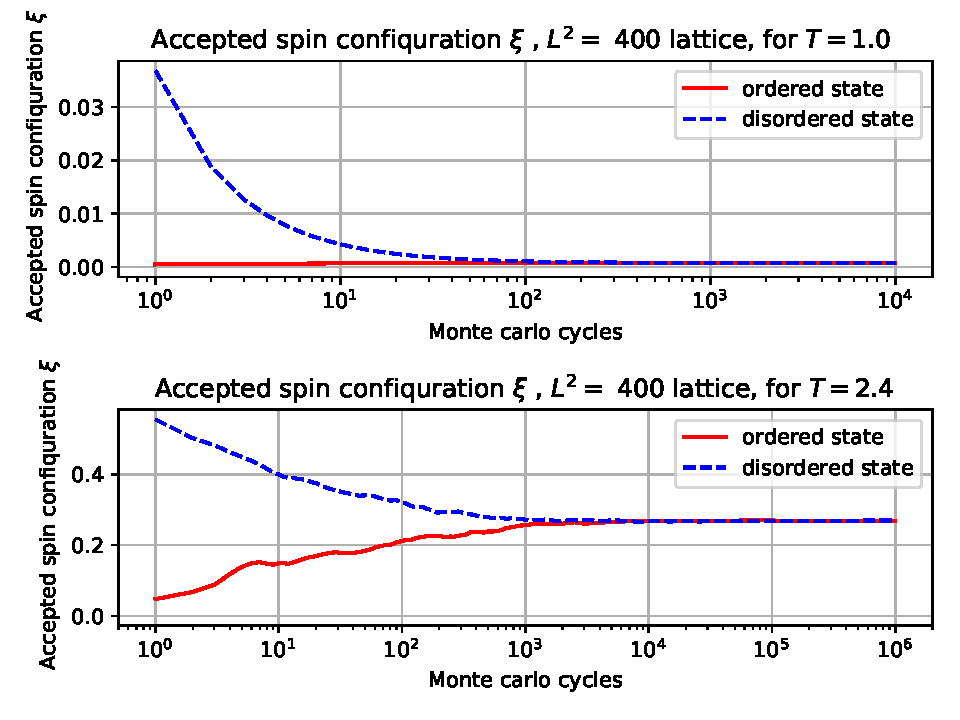
\includegraphics[width=17.0cm,height=6.3cm,keepaspectratio]{/Users/aramsalihi/Desktop/FYS4150/project4/figures/numerical_400_flipps_E_and_M_subplots.pdf}
  \centering
  \caption{A graph showing how number of accepted flips behave when number of Monte Carlo cycles increases.
  This is done for dis- and ordered system for temperature $kT/J = \{1.0,2.4\}$. The system achieves steady state at $10^{4}$ for $kT/J = 2.4$ and $10^{3}$ for $kT/J = 1.0$}
  \label{accept flips}
\end{figure}
\subsubsection{Probability density for $kT/J = 1.0$ and $kT/J = 2.4$ for disordered system}
\begin{figure}[H]
  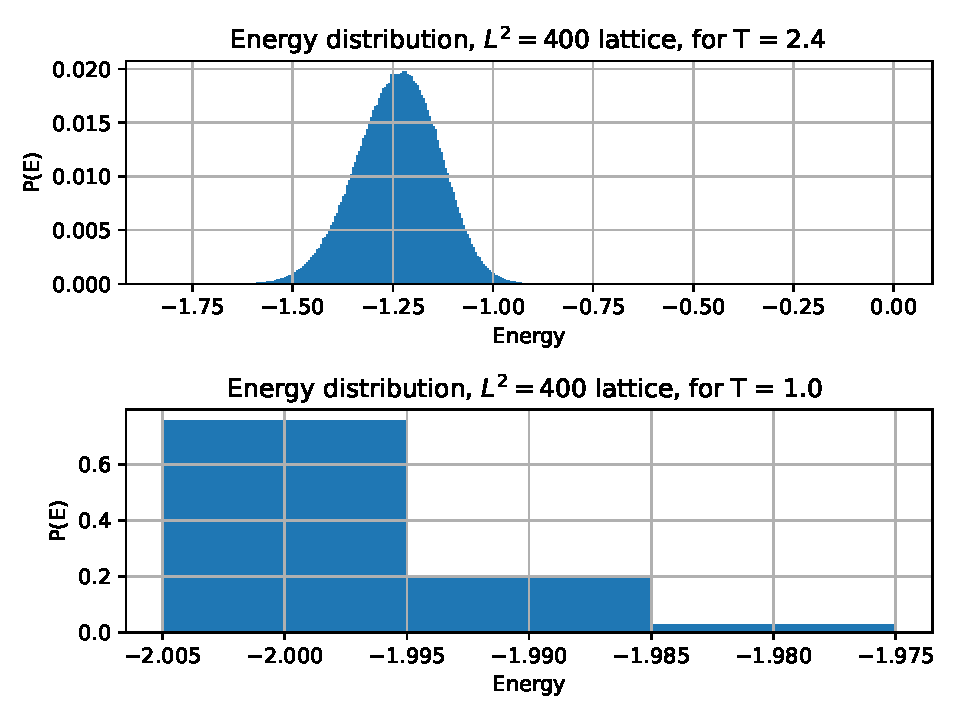
\includegraphics[width=17.0cm,height=6.3cm,keepaspectratio]{/Users/aramsalihi/Desktop/FYS4150/project4/figures/numerical_prob_dist_400_flipps_subplot.pdf}
  \centering
  \caption{The probability distribution of the energy for a disordered system. As described in the title, this has been done for
  the temperature $kT/J = \{1.0,2.4\}$.}
  \label{prob dist}
\end{figure}
\subsection{Phase transition for chaotic system for larger lattices}
In this subsection we are going to present the result when analyzing how a disordered system behaves after achieving
steady state near the Curie temperature for different lattice sizes. We used $L = \{40,60,80,100,120\}$. These simulations has been done on one node on the supercomputer "Abel" at the university of oslo.
We used $16$ cores in total with 64GB ram and executed $2e5$ Monte Carlo cycles per cores (in total $3.2e6$ Monte carlo cycles)
with a temeprature step $\Delta T = 0.01$ in the interval $kT/J = \{2.20,2.36\}$. Keep in mind that we have removed $625$ Monte Carlo cycles for each core,
this is due to that the system achieves steady after $625$ cycles (per core) and the real simulation starts after this point.
\subsubsection{Heat capacity and Magnetic susceptbility near Curie temperature}
\begin{figure}[H]
  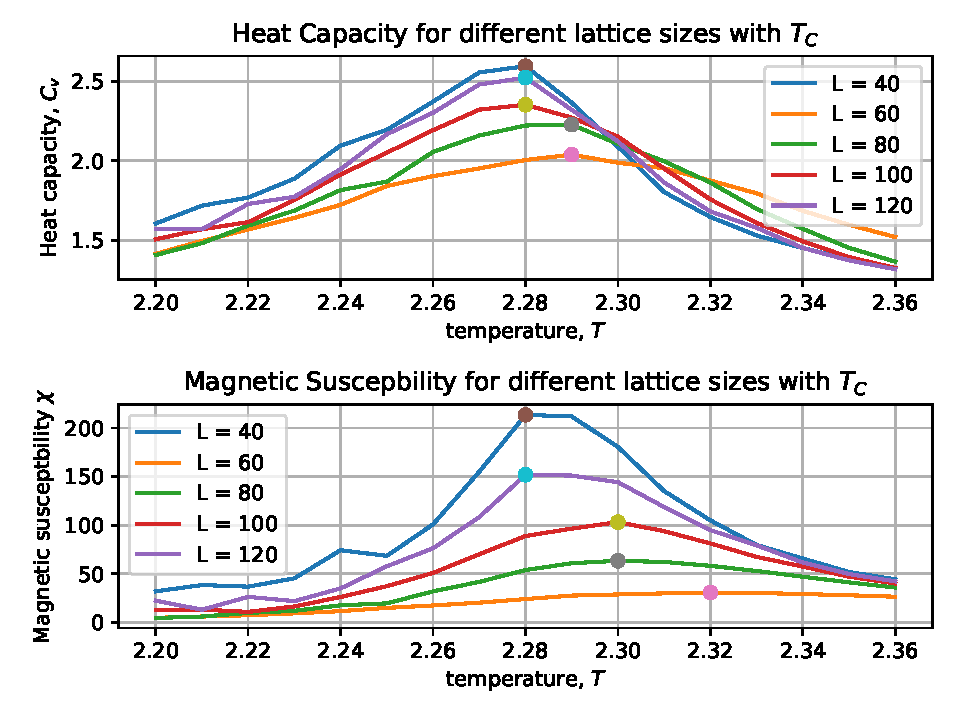
\includegraphics[width=17.0cm,height=6.3cm,keepaspectratio]{/Users/aramsalihi/Desktop/FYS4150/project4/figures/heatcap_magsus_subplot.pdf}
  \centering
  \caption{The behaviour of the heat capacity and magnetic susceptibility for different lattice sizes. Notice that the
  color points indicates where the Curie temperature occours for different lattice sizes.}
  \label{heatcap magsus}
\end{figure}
\subsubsection{Expectation value of absolute magnetic momenet and energy under phase transition}
\begin{figure}[H]
  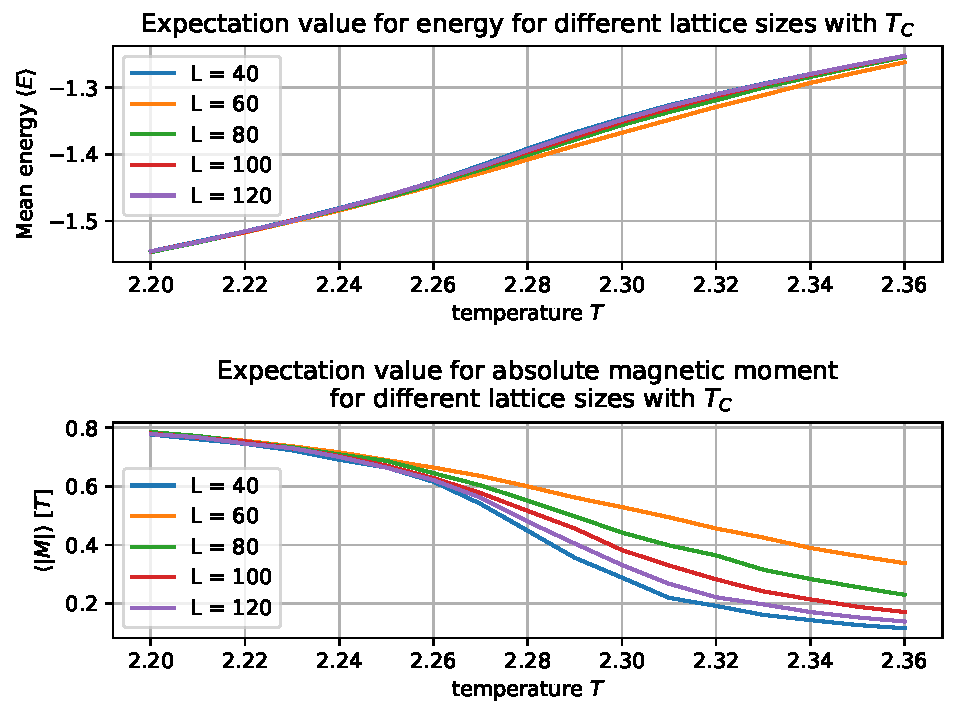
\includegraphics[width=17.0cm,height=6.3cm,keepaspectratio]{/Users/aramsalihi/Desktop/FYS4150/project4/figures/crit_subplot_meanE_meanM.pdf}
  \centering
  \caption{The behaviour of the expected energy and absolute magnetic moment when the system undergoes a second phase transition}
  \label{meanE fabsM Tc}
\end{figure}
\section{Discussion}
\subsection{$2\times 2$ lattice, analytical vs numerical solution}
Analyzing the result from $2\times 2$ lattice from subsection \eqref{2x2 result}, there was no suprise that the numerical
solution when increasing the number Monte Carlo cycle will converge towards the analytical solution found in subsection \eqref{2x2 analytical}.
This is a consequence of law of large number as explained in subsection \eqref{law of large numb}. Notice when analyzing figure \eqref{magsus og heatcap} and \eqref{meanE meanM},
that after $N = 1e6$  (where $5e5$ Monte Carlo cycles were distributed equaly between two cores
) we do get pretty good and accurate results. This result gives us an good indication on
how many Monte Carlo cycles it is needed to produce results with good precision. For larger systems than $20\times 20$ using $5e6$ per cores (if using two cores)
the computational time increases significantly, and therefore using $1e6$ total Monte Carlo cycles enough in order to save computational time.
\subsection{Time required to achieve steady-state} In this numerical study we refer time to number of Monte Carlo cycles needed to acheive stability.
As mentioned previous, we are heavily interested in how larger systems behave when increasing the lattice size. When increasing the lattice size, we also increase the computational time,
so therefore having a good knowledge on how the system behaves for different spin configuration and parameters is crucial.
\vspace{3mm}
\\
When analyzing figure \eqref{T = 1 20x20}, we notice that for a ordered spin oriented lattice (all spins points upward or downwars)
$\langle E \rangle$ starts very close to the expected value, the same goes with absolute magnetic moment. The explaination of this is that lattice is already
in the lowest possible state and therefore flipping spins is not required to achieve lower states. This observation and explaination is
supported by the first figure in \eqref{accept flips}. Analyzing this figure we notice that almost no spins are flipped. Looking at the energy distribution
for this system we notice that the lowest possible energy is around $\approx -1.9999$ with a probability of $\approx 0.80$.
Thus we obtain stability and steady state after $N = 10^{2}$ Monte Carlo cycles if using a ordered system. Meaning when calculating for large systems we can exclude the first $100$ steps if using ordered orientation, and then
look at the behaviour of the system.
\vspace{3mm}
\\
Analyzing the result further, we clearly notice there is a big difference between ordered and disordered spin states (all spins has randomly oriented orientation).
The explaination behind this behaviour: is that the lattice wants to achieve a stable spin orientation, thus the result will be either all spin pointing upwards or downwars.
When achieving this stable spin orientation, the lattice will be in the lowest possible state for $kT/J = 1$. A particle or a system of several particles always want to tend to
the lowest possible energy state. In this case the lowest possible energy is $\langle E \rangle \approx -1.9999$.
\vspace{3mm}
\\
Increasing the temperature to $kT/J = 2.4$ we get some interesting results, see figure \eqref{T = 2.4 20x20}.
When analyzing for the ordered lattice state, where each spin points upwards.
The system does not start as close to the expected energy $\langle E \rangle \approx -1.2486$,
but starts at a lower energy state $\approx -1.5897$. Which is relatively close, but not as close for the case with $kT/J = 1.0$.
From here the system take approximately
$N = 10^{4}$ Monte Carlo cycles in order to achieve lowest possible state and stability. The number of accepted spin flipps has
also significantly increased when analyzing \eqref{accept flips} and the number of
accepted spin stabilizes around $10^{4}$.
\vspace{3mm}
\\
Notice that the magnetic moment of the system
also decreases observed in figure \eqref{meanE fabsM Tc}. This obersvation is in depth
explained in subsection \eqref{ppp}. The explaination of this is that we will approach a
configruation where almost half of the spins are either oriented up,
and the other half oriented down. In this case we have some presentage of random oriented spin left, thus resulting in a lower
magnetic moment.
\vspace{3mm}
\\
When looking at the disordered system, a very interesting sight occours when looking
at the magnetic moment in figure \eqref{meanE fabsM Tc}. It appears it is almost zero,
it appears that we are more stable system. Meaning a large amount of spins starts in a configruation
where almost half of the spins are pointing up and the other pointing down. Notice that magnetic moment is not
zero, but very close. After few Monte Carlo cycles, $10^{2}$, the system is forced to approach another configruation in order
to achieve stability. It wants to balace out a
state with lower energy and a state with higher entropy.  This is a consequence
of Helmholtz free energy, thus the system wants to minimize this quantity. As we see the system then equilibriate itself and find
steady state after $10^{4}$ Monte Carlo cycles. Looking at the probability
distribution for this temperature and a disordered configuration in the lattice, we will observe
that the most likely energy is at $\approx -1.23475$. Which is actually the energy the lattice wants to end up in.
All in all for both temperatures is $10^{5}$ a very good amount of Monte Carlo cycles to
simulate since all quantitites are stabilized after $10^{4}$.

\subsection{Probability distribution}
Recall from figure \eqref{prob dist}, we see that probability distribution for the energy varies for different temperatures.
For $kT/J = 1$ the most desired state is when the expected energy is around $\approx -1.999$, this is the state where all spins point in the same direction.
The result of this that the expected magnetic moment is $\approx 0.9999$. For $kT/J = 2.4$ We get a spread, where the probability density is a almost gaussian distributed.
The highest and the most desired energy is $\approx -1.23548$ for this case, but still there spins with higher and lower energy than this.
This is due to not all of the spins are aligned in the same direction. There a few of them still randomly oriented.
The variance for $kT/J = 1.0$ is:
\begin{align}
  \sigma^{2}_{kT/J = 1} \approx 0.004220
\end{align}
and for $kT/J = 2.4$
\begin{align}
    \sigma^{2}_{kT/J = 2.4} \approx 0.001567
\end{align}
The standard deviation does not make sense for the case with $kT/J = 1.0$, and thus were ignored.
For the case $kT/J = 2.4$ the standard deviation were $\sigma \approx 0.03958$.

\subsection{Phase transition \label{ppp}} In this study we have analyzed the phase transition for five different lattices sizes.
As mentioned in subsection \eqref{phase transition} when the system gets closer to the Curie temperature, it undergoes a second phase transition.
Where thermodynamical quantities such as heat capacity and magnetic susceptibility is discontinous at $T_{c}$. This behaviour is observed in figure
\eqref{heatcap magsus}. After this point the system goes from
a ferromagnet to paramagnet, i.e looses its ability to self mangetize which can be oberserved in figure \eqref{meanE fabsM Tc}.
As you can see the magnetic moment tends to lower values, and becomes zero for some temperature values, $T >> T_{c}$. The convergence is heavily dependent on the lattice size. The
bigger lattice the faster the magnetic moment converges towards zero. As consequence of this, the energy of the system increases because
after a while when system stabilizes half of the spins is oriented up and the other half pointing down. This gives a higher energy, and the magnetic moment dies out
for large temperatures. Thus becoming a paramegnet. The estimated Curie temperature for these
five lattices are given in the table down below
\begin{table}[H]
  \centering
  \begin{tabular}{cccccc}\toprule
    $L$ & $T_{C}$ & $C_{v}$ & $\chi$ &
    \\ \midrule
    $40$ &  $2.28$ & $2.60$ & $213.43944$ \\
    $60$ &  $2.32$ & $1.88$ & $30.675726$ \\
    $80$ &  $2.30$ & $2.11$ & $63.38758$ \\
    $100$&  $2.30$ & $2.20$ & $103.19285$ \\
    $120$&  $2.28$ & $2.52$ & $151.86274$\\
    \bottomrule
  \end{tabular}
  \caption{This table list the value of the heat capacity and magnetic
  susceptbility at $T_{c}$ for different lattice sizes with spin $L$.
  There is a minimal difference in $T_{c}$ for the heat capacity and magnetic susceptbility
  where the discontinuity occours}
  \label{tabell}
\end{table}
The main goal of this numerical study where to estimate the Curie temperature and to get a better understanding of the phenomena
, using the produced result and recall the constant $a$ in \eqref{a}
\begin{align}
    a = \frac{T_{C}(L_{1}) - T_{C}(L_{2})}{L_{1}^{-1/\nu}-L_{2}^{-1/\nu}}
\end{align}
Using $L = 120$ and $L = 60$ with $\nu = 1$, we can estimate this constant to be
\begin{align}
  a \approx 4.8
\end{align}
And using \eqref{curie temp relation} for $L = 120$, we get that
\begin{align}
  T_{C}(L \to \infty) = 2.28- \frac{4.8}{120} \approx 2.24
\end{align}
The theoretical predicted by Onsager is $\approx 2.269$. Using this we can calculate the relative error is
\begin{align}
  \epsilon_{rel} = 100\%\frac{|2.269-2.24|}{2.269} \approx 1.278\%
\end{align}
Which is acceptable. We could have achieved quite significantly much better $T_{C}$ result if we choose to use smaller than $\Delta T = 0.01$.
The problem is we need to increase the number of Monte Carlo cyclus, thus the computational time increases significantly. For this run, we runned
16 cores on one node on the super computer ABEL. We used in total $3.2e6$ Monte Carlo cycles, where each core took $2e5$ cycles. All in all the acceptable result is
\begin{align}
    T_{C}(L \to \infty) \approx 2.24 \pm 0.029
\end{align}
\section{Conclusion}
Our goal of this numerical study was to get a better understanding of what happens with our system when it nears
the Curie temperature. As it turns out the system after $T_{C}$ the system magnetic moment converges toward zero for large temperature. Thus resulting in
higher energy states which also approach zero for higher temperatures. This is due to that the material has spins where half of the spins are pointing upwards and the other half down,
this result in increase of energy for individual spin, resulting a higher energy state for the lattice. The conclusion is that the system goes from
a ferromagnetic system to paramagnetic system.
\vspace{3mm}
\\
In general we have found out that in order to achieve a stable and steady state system, we only require to perform
$N = 10^{4}$ Monte Carlo cyclus. For larger system the computational time increases significantly since we need to go through every
spin particles in the lattice, therefore it is crucial to have good understanding of how the different type of thermodynamical quantities converges.
It is good to use $10^{5}$ Monte Carlo cycles for large system, eventhough we used $3.2e6$, but this was due to
accessbility on a better computer, and we took the chance to improve our data. Further, we also found the analytical solution of
$2\times 2$ lattice.
\bibliographystyle{apalike}
\bibliography{project4}
\newpage
\section{Appendix A: Derivation of heat capacity \label{heat capacity}}
In this section we are going to derive the relation:
\begin{align}
  C_{v} = \frac{\mathrm{Var}(E)}{kT^{2}}
\end{align}
Consider the following mathematical definition of heat capacity
\begin{align}
  C_{v} = \pdv{\langle E \rangle}{T}
\end{align}
Before we start to derive this equation it is useful to derive the expectation values of energy and energy squared.
Consider
\begin{align}
  \langle E \rangle = \frac{1}{Z}\sum_{i}E_{i} e^{-\beta E_{i}} = -\pdv{\beta}\ln{Z}
  \label{1}
\end{align}
and
\begin{align}
  \langle E^{2} \rangle = \frac{1}{Z}\sum_{i}E_{i}^{2} e^{-\beta E_{i}}
  \label{2}
\end{align}
 Notice that the parition function is $Z = \sum_{i} e^{-\beta E_{i}}$, meaning if we differentiate
 $Z$ with respect to the boltzman factor $\beta$, we will obtain \eqref{1} times the inverse of $Z$. If we second differentiate $Z$ with respect
 to the boltzman factor, we will acieve \eqref{2} times the inverse of $Z$. Thus we can write
 \begin{align}
     \langle E \rangle = \frac{1}{Z} \pdv{Z}{\beta}
 \end{align}
 And
 \begin{align}
   \langle E^{2} \rangle = \frac{1}{Z} \pdv[2]{Z}{\beta}
\end{align}
Going back to the definition of heat capacity, and use the expectationv value of the energy, we can write
\begin{align}
    C_{v} = \pdv{\langle E \rangle}{T} = - \pdv{T}\pdv{\beta}\ln{Z} = - \pdv{T}\left( \frac{1}{Z}\sum_{i}E_{i} e^{-\beta E_{i}} \right)
\end{align}
Differentiating this and performing the chain rule
\begin{align}
    C_{v} = -\frac{1}{Z^{2}}\sum_{i}E_{i}e^{-\beta E_{i}}\pdv{Z}{T} + \frac{1}{Z}\sum_{i}\frac{E^{2}}{kT^{2}}e^{-\beta E_{i}}
\end{align}
The term
\begin{align}
  \pdv{Z}{T} = \sum_{i}\frac{E_{i}}{kT^{2}}e^{-\beta E_{i}}
\end{align}
Using this in our expression, we have
\begin{align}
    C_{v} = -\frac{1}{kT^{2}}\left(\frac{1}{Z^{2}}\sum_{i}E_{i}e^{-\beta E_{i}}\right)^{2}
    + \frac{1}{kT^{2}}\left(\frac{1}{Z}\sum_{i}e^{-\beta E_{i}}\right)
\end{align}
Notice that first term is just sqaured expectation value of the energy, and the second term is just expectation value of the energy squared.
Thus
\begin{align}
  C_{v} = \frac{1}{kT^{2}}\left(\langle E^{2} \rangle - \langle E \rangle^{2}\right) = \frac{\mathrm{Var}(E)}{kT^{2}}
\end{align}
\section{Appendix B: Derivation of Magnetic susceptibility \label{magnetic susceptibility}} In this section we are going derive the relation between
magnetic susceptbility and the variance of the magnetic moment. Consider the definiton of magnetic susceptibility
\begin{align}
\chi = \pdv{\langle M \rangle}{B}
\end{align}
Where $B$ is the magnetic field strength. Using the definition of expectation value
on the magnetic moment, we can write this as:
\begin{align}
  \chi = \pdv{B}\left(\frac{1}{Z}\sum_{i}M_{i}e^{-\beta E_{i}}\right)
\end{align}
If we assume the general case where the energy states can be written as
\begin{align}
  E_{i} = \epsilon_{i} - M_{i}B
\end{align}
Where $\epsilon$ is the energy from \eqref{ising energy} and $M_{i}$ is the magnetic moment.
Thus
\begin{align}
  \chi = \pdv{B}\left(\frac{1}{Z}\sum_{i}M_{i}e^{-\beta(\epsilon_{i} - M_{i}B)}\right)
\end{align}
Now differentiating this with respect to the magnetic field strength $B$ by using the product and chain rule, we will achieve the
following
\begin{align}
  \chi = -\underbrace{\frac{\beta}{Z^{2}}\sum_{i}M_{i}^{2}e^{-\beta ( \epsilon_{i} - M_{i}B)}}_{\langle M \rangle^{2}}
  + \underbrace{\frac{\beta}{Z}\sum_{i}M_{i}^{2}e^{-\beta ( \epsilon_{i} - M_{i}B)}}_{\langle M^{2} \rangle}
\end{align}
This is just
\begin{align}
  \chi = \frac{\langle M^{2} \rangle - \langle M \rangle^{2}}{kT} = \frac{\mathrm{Var}(M)}{kT}
\end{align}
Which another expression for the magnetic susceptibility.
\end{document}
